\documentclass[a4paper]{article}

% Pacotes para o português.
\usepackage[brazilian]{babel}
\usepackage[utf8]{inputenc}
\usepackage[T1]{fontenc}

\usepackage{datetime}
\usepackage{graphicx}

% Usado nos pedaços de código.
\usepackage{listings}
\lstset{language=C,
	basicstyle=\small\sffamily,
	numbers=left,
	numberstyle=\tiny,
	frame=tb,
	columns=fullflexible,
	showstringspaces=false,
	captionpos=b}
\renewcommand\lstlistingname{Código}

\newcommand{\HRule}{\rule{\linewidth}{0.5mm}}

\begin{document}

\begin{titlepage}
\begin{center}	

% Topo 1.
\textsc{\Large UNIVERSIDADE DE SÃO PAULO\\
	INSTITUTO DE CIÊNCIAS MATEMÁTICAS E DE COMPUTAÇÃO}\\[0.7cm]

% Topo 2.
\textsc{\Large SSC0143}\\[0.2cm]
\textsc{\Large Programação Concorrente - Turma B}\\[0.5cm]

% Título.
\HRule \\[0.4cm]
{ \huge \bfseries Projeto da Disciplina}\\[0.4cm]
\HRule \\[0.4cm]
\textsc{Professor Dr. Julio Estrella}\\[1.5cm]

% Grupo
\begin{minipage}{0.4\textwidth}
\begin{flushleft} \large
\emph{Grupo 06:}\\
Bruno Junqueira Adami\\
Lucas Junqueira Adami\\
Lucas Lobosque\\
\end{flushleft}
\end{minipage}
\begin{minipage}{0.4\textwidth}
\begin{flushright} \large
\emph{Números USP:}\\
6878762\\
6792496\\
6792645\\
\end{flushright}
\end{minipage}

\vfill

% Rodapé.
{\large \today}
	
\end{center}
\end{titlepage}

\section{Introdução}
\indent \indent Este projeto consiste em desenvolver uma aplicação paralela que gere palavras aleatoriamente. A cada palavra gerada, deve-se verificar se ela está no dicionário de entrada. Caso ela esteja, ela deve ser removida. A aplicação acaba quando todas as palavras são geradas. Há várias maneiras de abordar o que foi proposto. Portanto, a interpretação que foi adotada será explicada neste documento.\\
\indent O projeto consiste de três módulos: a filtragem do dicionário, a geração das palavras aleatórias e a busca e remoção no dicionário. Palavras inteiras de tamanho 5 são geradas e depois é efetuada uma verificação da existência delas no dicionário. Caso uma palavra gerada exista, é removida e impressa na tela. Para palavras de tamanho menor do que 5, são comparadas as primeiras letras. Como podem existir vários prefixos de palavras iguais (Ex: abcde, abc), é escolhida a palavra de tamanho maior primeiro. Caso haja empate, a primeira que foi carregada do dicionário será escolhida. As palavras de tamanho maior do que 5 são divididas em várias palavras de tamanho 5 onde, depois de gerada uma destas partes, é verificado se todas as outras partes desta palavra composta foram geradas. Caso positivo, ela é mostrada na tela. Essa decomposição está melhor explicada nas próximas seções.

\section{Filtragem do Dicionário}
\indent \indent O dicionário de entrada fornecido no site da disciplina foi filtrado. Um programa serial que carrega as palavras eliminando as letras inválidas (vírgulas, espaços e outros símbolos) foi desenvolvido. Além disso, foi efetuada uma identificação e eliminação de palavras repetidas. Para desenvolver tal programa, uma árvore de prefixos foi implementada, conhecida como \emph{trie}. Ela é uma árvore onde cada ramo representa uma letra de ramificação da palavra. A complexidade de inserção e busca nesta estrutura de dados é de \begin{math}O(n)\end{math}, onde \begin{math}n\end{math} é o tamanho da \emph{string} a ser inserida. A complexidade é linear (\begin{math}O(n)\end{math} onde \emph{n} é o tamanho de todas as palavras somadas) na leitura do arquivo e na manipulação da \emph{trie}. A complexidade em memória também é de \begin{math}O(n)\end{math}, onde \emph{n} é o tamanho de todas as palavras somadas, pois cada nó aloca dinamicamente os ramos da árvore.\\
\indent No final da filtragem, há a produção de um arquivo com as palavras do dicionário com letras de a-z apenas, uma em cada linha. No total, o arquivo tem 65813 palavras e um tamanho de 616\emph{KB}.

\section{Separação do Problema em Vários \emph{Hosts}}
\indent \indent  Um dos requisitos do projeto é o de usar os \emph{hosts} do \emph{cluster} da disciplina para fazer o processamento do problema. Para isso é utilizado a biblioteca \emph{MPI}. Duas abordagens possíveis foram estudadas. A primeira é de alguma forma compartilhar todo o dicionário para todos os nós e sincronizar a remoção de palavras geradas do mesmo. Isso causa um enorme tráfego na rede e esta abordagem foi descartada. A segunda, adotada no projeto, é separar o dicionário em cada \emph{host}. As palavras compostas devem ficar nos mesmos \emph{hosts} para evitar a comunicação entre os nós, aumentando a eficiência da abordagem. Na separação do dicionário não há nenhum \emph{speedup} (negativo ou positivo), pois como as palavras são geradas aleatoriamente (uniformemente), a probabilidade a cada ciclo de execução de uma palavra ser removida do dicionário é a mesma.\\
\indent Suponha que há \emph{M} palavras todas de tamanho 5 no dicionário. Suponha que a probabilidade de cada palavra sair seja \begin{math}1/26^5\end{math}. A probabilidade em um passo de gerar alguma palavra do dicionário é de \begin{math}M/26^5\end{math}. Se o dicionário for separado entre três nós, \begin{math}A\end{math} palavras para o primeiro, \begin{math}B\end{math} para o segundo e \begin{math}C\end{math} para o terceiro, a esperança (média) de palavras geradas é de \begin{math}A/26^5 + B/26^5 + C/26^5\end{math}, ou \begin{math}(A+B+C)/26^5\end{math}. Como \begin{math}A+B+C = M\end{math}, a probabilidade para três nós é a mesma probabilidade para um nó.\\
\indent Ao incluir palavras de tamanho menor, a demonstração fica um pouco mais complexa, mas o resultado é o mesmo. Na prática foi testado se essa suposição matemática está correta, e foi comprovado que o \emph{speedup} é de 1. Também foi testada a mesma teoria no próprio nó e o mesmo foi observado. Portanto, o \emph{speedup} do problema deve ser focado em cada nó. Ou seja, onde é separado o problema no próprio \emph{host}. Ao alcançar um \emph{speedup} de X em cada nó, o \emph{speedup} total será de \begin{math}X*Y + T\end{math} onde \begin{math}Y\end{math} é a quantidade de nós e \begin{math}T\end{math} o tempo inicial para separar as palavras em cada \emph{host}.

\section{Geração das Palavras Aleatórias}
\indent \indent Do primeiro trabalho, na geração de números aleatórios para fazer o método de \emph{Monte Carlo}, já era sabido que a função \emph{rand} da \emph{stdlib} no \emph{C}, na implementação da \emph{libC} no \emph{Linux}, usa de travamentos de contexto para gerar o número aleatório. Então, um novo gerador de números aleatórios foi criado. Um gerador congruente linear foi desenvolvido, com os parâmetros personalizados para o problema:
\begin{eqnarray*}
	M = 11881376 \\\textrm{são \begin{math}26^5\end{math} palavras possíveis de tamanho 5}\\
	A = 53\\
	C = 3\\
\end{eqnarray*}	
\indent Os parâmetros \emph{A} e \emph{C} devem obedecer as restrições dadas em \cite{random2}. Também, um programa para testar se realmente o gerador é uniforme foi criado. Se a geração ocorrer letra a letra, a probabilidade de se gerar uma palavra de tamanho 5 qualquer é de \begin{math}1/26^5\end{math}. Ao invés de gerar letra a letra, a palavra foi representada como um número de tamanho 5 na base 26 (0-11881376). São \begin{math}26^5\end{math} números e cada um tem a mesma chance de ser escolhido (geração uniforme). Assim a probabilidade é de \begin{math}1/26^5\end{math}, a mesma na geração letra a letra.

\section{Processamento do Problema em Cada \emph{Host}}
\indent \indent Agora há em cada nó o mesmo problema. Dado o dicionário, gerar palavras de tamanho 5 aleatoriamente e remover as encontradas até que não exista mais palavras. Inicialmente, a \emph{trie} foi adotada para representar o dicionário, pois foi utilizada na filtragem da entrada e ela é uma estrutura simples e eficiente. Então, de algum modo é preciso paralelizar as funções de busca e remoção nesta estrutura.\\
\indent Para paralelizar o problema em cada nó a \emph{Pthreads} foi utilizada, pois esta \emph{API} fornece uma programação bem mais baixo nível em relação a \emph{OpenMP}. Isto não significa que o problema não pode ser paralelizado usando \emph{OpenMP}. A adoção dessa \emph{API} foi uma escolha de projeto.\\
\indent Como a \emph{trie} é uma árvore de prefixos, o modo mais intuitivo de fazer estas funções é com buscas em profundidade. Porém, na criação de mais de uma unidade de processamento para fazer a busca, é necessário garantir que os nós estejam sincronizados. Na prática, foi preciso inserir vários trancamentos de contextos (\emph{mutex locks}) e o resultado não foi satisfatório. Também, uma abordagem de busca em largura nesta árvore foi pensada. Mas, antes de pô-la em prática foi decidido que a árvore não era realmente a estrutura mais fácil e eficiente disponível para resolver o problema.\\
\indent Então, foi discutido que a solução ótima é a utilização de \emph{hashing}. O número aleatório de tamanho 5 na base 26 gerado pelo gerador linear congruente gera uma \emph{hash} para a palavra, tornando o problema muito simples:
\begin{eqnarray*}
	funcaoHash(str) = 26^0*(str[0] - 'a') + 26^1*(str[1] - 'a') + 26^2*(str[2] - 'a')\\
	+ 26^3*(str[3] - 'a') + 26^4*(str[4] - 'a')
\end{eqnarray*}
\indent Cada \emph{thread} gera uma \emph{hash} que representa uma palavra de tamanho 5. Se essa \emph{hash} existe no dicionário então é retirada da estrutura. Observe que não há colisões neste \emph{hash}. O dicionário é um vetor de inteiros de tamanho \begin{math}26^5\end{math}, onde cada posição indexa o \emph{hash} da \emph{string} e quantas delas existem. Em torno de 40\emph{MB} de memória é utilizado, muito maior do que a \emph{trie}. Porém, a complexidade de busca/remoção na execução é de \begin{math}O(1)\end{math}. Para sincronizar as \emph{threads} que geram essas \emph{hashes} os travamentos de contexto foram utilizados e o resultado foi de um \emph{speedup} de 4 (testado em uma máquina com 4 \emph{CPUs}). Para montar o dicionário no começo do programa, a complexidade em tempo é a mesma do que a \emph{trie}, pois o cálculo da \emph{hash} da palavra é linear no tamanho dela. O \emph{speedup} será proporcional ao número de \emph{hosts} vezes o número de unidades de processamento de cada \emph{host}.

\section{Palavras de Tamanho Diferente de 5}
\indent \indent O dicionário tem uma separação por tamanho de palavras. Ou seja, ele tem uma partição para palavras de tamanho 5, outra para as de 4 e assim até as de tamanho 1. Não é possível tratar o \emph{hash} de palavras de tamanho 5 com de outros tamanhos (Ex: \begin{math}hash("aaaaa") = 0\end{math}, \begin{math}hash("a") = 0\end{math}). Portanto, após gerar uma \emph{hash} randômica, é verificado primeiro as palavras de tamanho 5, depois 4 e assim em diante.\\
\indent Um outro problema é o que fazer com as palavras de tamanho maior do que 5. Na especificação do projeto foi decidido que palavras maiores do que este número devem ser quebradas em várias palavras, por causa da probabilidade de se gerar uma palavra de tamanho grande, por exemplo 7: \begin{math}1/26^7 \simeq 8*10^9\end{math}. Esse número cresce exponencialmente à medida que o tamanho da palavra cresce.\\
\indent A solução desenvolvida quebra essas palavras em palavras de tamanho 5 (ou menos caso for a última parte) e atribui à elas um identificador e qual parte da palavra toda esta pequena parte representa. As palavras de tamanho menor ou igual a 5 também receberão um identificador e elas representam toda a palavra. Há um vetor global que guarda as informações de todas as palavras, indexado pelo identificador da palavra. Cada posição guarda qual palavra é, quantas partes tem e quais já foram sorteadas. Esse vetor nada mais é do que um complemento do dicionário como um todo. As partes das palavras recebem uma máscara que devem \emph{setar} no vetor global de informações caso sejam sorteadas. Irão existir várias palavras com o mesmo prefixo. Foi interpretado que deve-se gerar o número de vezes que este prefixo aparece, e não apenas uma vez, já que a própria versão sequencial neste caso leva menos do que 2 segundos para executar.\\
\indent Por exemplo a palavra "aaaaaba". Ela deve ser separada em "aaaaa" e "ba". Portanto há uma máscara de 2 partes, ou seja, 2 bits. A primeira parte ("aaaaa") deve \emph{setar} o primeiro bit (1 em decimal ou 01 em binário). Isto é, realizar a operação \emph{or} com a máscara no vetor de informações. A segunda parte ("ba") deve \emph{setar} o segundo bit (2 em decimal ou 10 em binário). Ela também realiza o \emph{or} com a máscara no vetor de informações. Quando o número de bits \emph{setados} for igual ao número de partes, significa que a palavra foi totalmente gerada.
\begin{eqnarray*}
	\textrm{vetor global das palavras} \rightarrow \textrm{id: 0 palavra: "aaaaaba" \quad partes: 2 máscara: 0}\\
	\textrm{dicionário indexado pelo hash} \rightarrow \textrm{hash: 0 id\_palavra: 0 máscara: 1}\\
					 \textrm{hash: 1 id\_palavra: 0 máscara: 2}\\
\end{eqnarray*}	
\indent Podem existir mais de uma palavra de tamanho 5 (ou outros tamanhos), representando partes de palavras diferentes. Será escolhido o que primeiro foi adicionado no dicionário. No final, o tempo total de geração das palavras será o mesmo.
	
\section{Resultados e Conclusões}
\indent \indent Uma execução em uma máquina local foi feita para comprovar que a suposição sobre a separação do problema em vários \emph{hosts} é proporcional ao \emph{speedup} em cada nó. Para isso o arquivo do dicionário foi separado em duas, quatro e oito partes e foi executado a versão com uma \emph{thread} em cada um destes pedaços do dicionário. Portanto, o \emph{speedup} é da ordem de 1:	
\begin{itemize}
	\item 1 parte: 4m5.889s
	\item 2 partes: 2m17.614s + 1m50.646s = 4m8.260s
	\item 4 partes: 1m16.884s + 0m51.535s + 0m43.798s + 1m31.629s = 4m23.846s
	\item 8 partes: 0m49.536s + 0m39.686s + 0m34.536s + 0m19.279s + 0m24.148s + 0m22.988s + 0m39.004s + 0m35.433s = 4m24.610s
\end{itemize}
\indent É possível observar uma pequena diferença entre os tempos devido à inicialização do programa. Porém, o \emph{speedup} observado foi realmente de 1.\\
\indent Depois, foi executada a versão final (paralela) no \emph{cluster} da disciplina com 4 \emph{threads} em cada \emph{host}, tirando uma média entre 10 repetições. O resultado se encontra na Figura~\ref{pic-graph}. O gráfico mostra os números de nós utilizados e seus respectivos tempos de execução. Fica comprovado que toda a teoria desenvolvida anteriormente sobre o problema está correta, já que o \emph{speedup} foi proporcional ao número de \emph{hosts}.\\
\begin{figure}[float=h!]
	\centerline{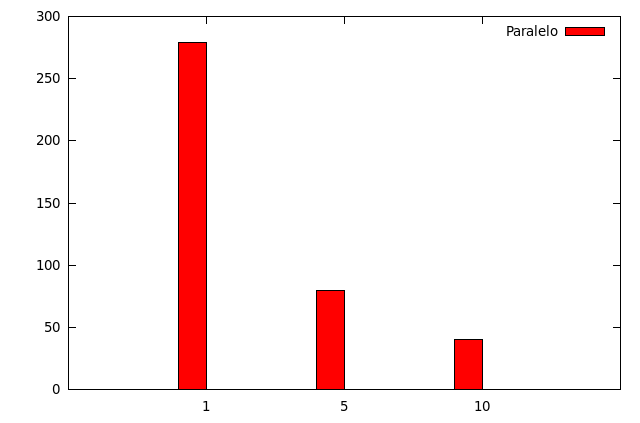
\includegraphics[width=285px, height=215px]{graph}}
	\caption{Execuções no \emph{cluster}}
	\label{pic-graph}
\end{figure}

\indent É possível concluir que muitas vezes a melhor solução para o problema sequencial não é totalmente aplicável e/ou pode se tornar facilmente paralela. É necessário analisar os vários pontos de vista de um problema. A solução pode ser mais fácil do que parece e, neste caso, já estava implementada de uma maneira indireta na geração de palavras aleatórias.

\begin{thebibliography}{99}

	\bibitem[Probabilidades]{prob}http://mathworld.wolfram.com/DiscreteUniformDistribution.html
	\bibitem[Random]{random}http://pubs.opengroup.org/onlinepubs/009695399/functions/rand.html
	\bibitem[Random]{random2}http://en.wikipedia.org/wiki/Linear\_congruential\_generator
	\bibitem[GLibC]{glibc}http://www.gnu.org/software/libc/download.html
	\bibitem[PThreads]{pth1}http://en.wikipedia.org/wiki/Native\_POSIX\_Thread\_Library
	\bibitem[PThreads]{pth2}http://www.icir.org/gregor/tools/pthread-scheduling.html
	\bibitem[PThreads]{pth3}http://www.yolinux.com/TUTORIALS/LinuxTutorialPosixThreads.html
	\bibitem[Trie]{trie}http://www.cs.bu.edu/teaching/c/tree/trie/
	\bibitem[Hashing]{hash}http://ocw.mit.edu/courses/electrical-engineering-and-computer-science/6-046j-introduction-to-algorithms-sma-5503-fall-2005/video-lectures/lecture-7-hashing-hash-functions/
	\bibitem[Hashing]{hash2}http://ocw.mit.edu/courses/electrical-engineering-and-computer-science/6-046j-introduction-to-algorithms-sma-5503-fall-2005/video-lectures/lecture-8-universal-hashing-perfect-hashing/
	\bibitem[Hashing]{hash3}http://research.cs.vt.edu/AVresearch/hashing/strings.php
	\bibitem[MPI]{mpi1} http://www.slac.stanford.edu/comp/unix/farm/mpi.html
	\bibitem[MPI]{mpi2} http://www.eecis.udel.edu/\~{}saunders/courses/372/01f/manual/manual.html
	\bibitem[Gnuplot]{gnuplot}http://www.duke.edu/~hpgavin/gnuplot.html
	
\end{thebibliography}
\end{document}
